
This lecture introduces more manifold learning algorithms including
Isomap, LLE, LE, MVU and briefly mentions an analog of JL-lemma in the
manifold setting. 

\section{Non-Linear Dimensionality Reduction}
So far, we've been trying to minimize $||X-UV||_F^2$ with  $U\in \mathbb{R}^{D\times d}$ and $V\in \mathbb{R}^{d\times n}$. In this case, $U$ is modeling a linear combination. But if we have $X=f(V)$ instead, where $f$ is a non-linear, smooth function, then we have a non-linear combination. \\
For example, consider a robot moving its head with angle $\theta$. The image at each angle would be a vector in $\R^{100 \times 100}$. Then, in this case we can learn a mapping from $\theta$ to a vector in $\R^{100 \times 100}$. $\theta$ would be the low-dim representation in this case.\\

\textbf{Idea}: Underlying data follows some kind of manifold. \\

\textbf{Manifold} is a set of points which locally resembles Euclidean space. Specifically, manifold is a topological space such that for each point on manifold, the local neighborhood is homeomorphic to Euclidean space. \textbf{Homeomorphic} means that there exists a continuous bijection that maps from the local neighborhood to the Euclidean space. \\

Agenda for today:
\begin{itemize}
\item Isomap (Isometric mapping)
\item LLE (Locally Linear Embedding)
\item LE (Laplacian Eigenmaps)
\item MVU (Maximum Variance Unfolding)
\item kernel PCA
\item Some open problems and approaches to solve these problems
\end{itemize}

\subsection{Isomap}
\subsubsection*{Goal}
To represent large dimensional data in low dimension, such that global geometry of the manifold is preserved. Applications: computer vision. \\
Question: What is global geometry? The geodesic distances between data points. 

\subsubsection*{Notation}
Input data is $X \in \mathbb{R}^{D\times n}$. Output data $Y \in
\mathbb{R}^{d\times n}$ where $d\ll D$. 

\subsubsection*{How?}
\begin{itemize}
\item Approximate the geodesic distances by computing the shortest
  path on a $k$-nearest neighbor ($k$-NN) graph constructed on the input data
  (note that the $k$-NN graph needs to be connected). Use ASSP (All Source Shortest Path algorithm) to compute the shortest paths.
\item Construct a "distance" matrix $D^{(G)}_{n\times n}$.
\item Run (classical/metric) MDS (multidimensional scaling) on $D^{(G)}_{n\times n}$ to find
  the corresponding low dimension embedding of $X$ ($\min_{Y} \sum_{i<j}||y_i - y_j|| -
  D^{(G)}_{ij}$). 
  
 \item The number of sample points is usually $O(Vk^d)$ where $V$ is volume and $k,d$ are curvature and intrisic dim respectively. 
\end{itemize}

\begin{figure}
\centering
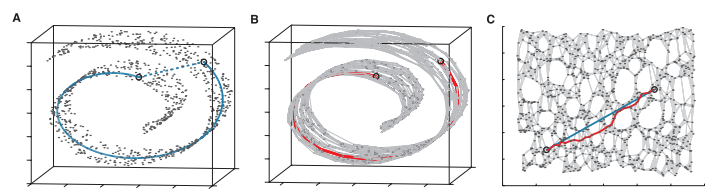
\includegraphics[width=0.7\textwidth]{chapter_7/files/isomap.png}
\caption{Illustration of geodesic distance}
\end{figure}


\subsubsection*{Observations}
\begin{itemize}
\item How well can $k$-NN graph approximate the geodesics.
  \begin{itemize}
  \item Under suitable distributions over the underlying    manifold,
    as $r\rightarrow 0$, $n\rightarrow \infty$, $nr \rightarrow
    \infty$, we can show that ASSP approximates the geodesics. 
  \end{itemize}
 
\begin{figure}
\centering
\begin{tikzpicture}
\draw (2,2) circle (1.5cm);
\draw (10,2) arc[x radius=1.5, y radius=1.5, start angle=0, end angle=-350];
\end{tikzpicture}
\caption{A circle (manifold), as shown on the left, cannot be properly mapped to $\mathbb{R}^{1}$. But if we have a hole, as shown on the right, then it can be embedded to $\mathbb{R}^{1}$. } \label{fig:M1}
\end{figure}
 
\item For what kinds of manifolds does Isomap work? When can geodesic paths become Euclidean paths?
  \begin{itemize}
  \item Underlying manifold needs to be (globally) isometric to some Euclidean space 
    $\mathbb{R}^n$; that is, it has no intrinsic curvature. For
    example, a spherical cap (a hemisphere) cannot be embedded into
    Euclidean space without distorting distances (imagine trying to
    flatten the northern hemisphere of a globe without
    stretching/ripping the map).  
    
\begin{figure}
\centering
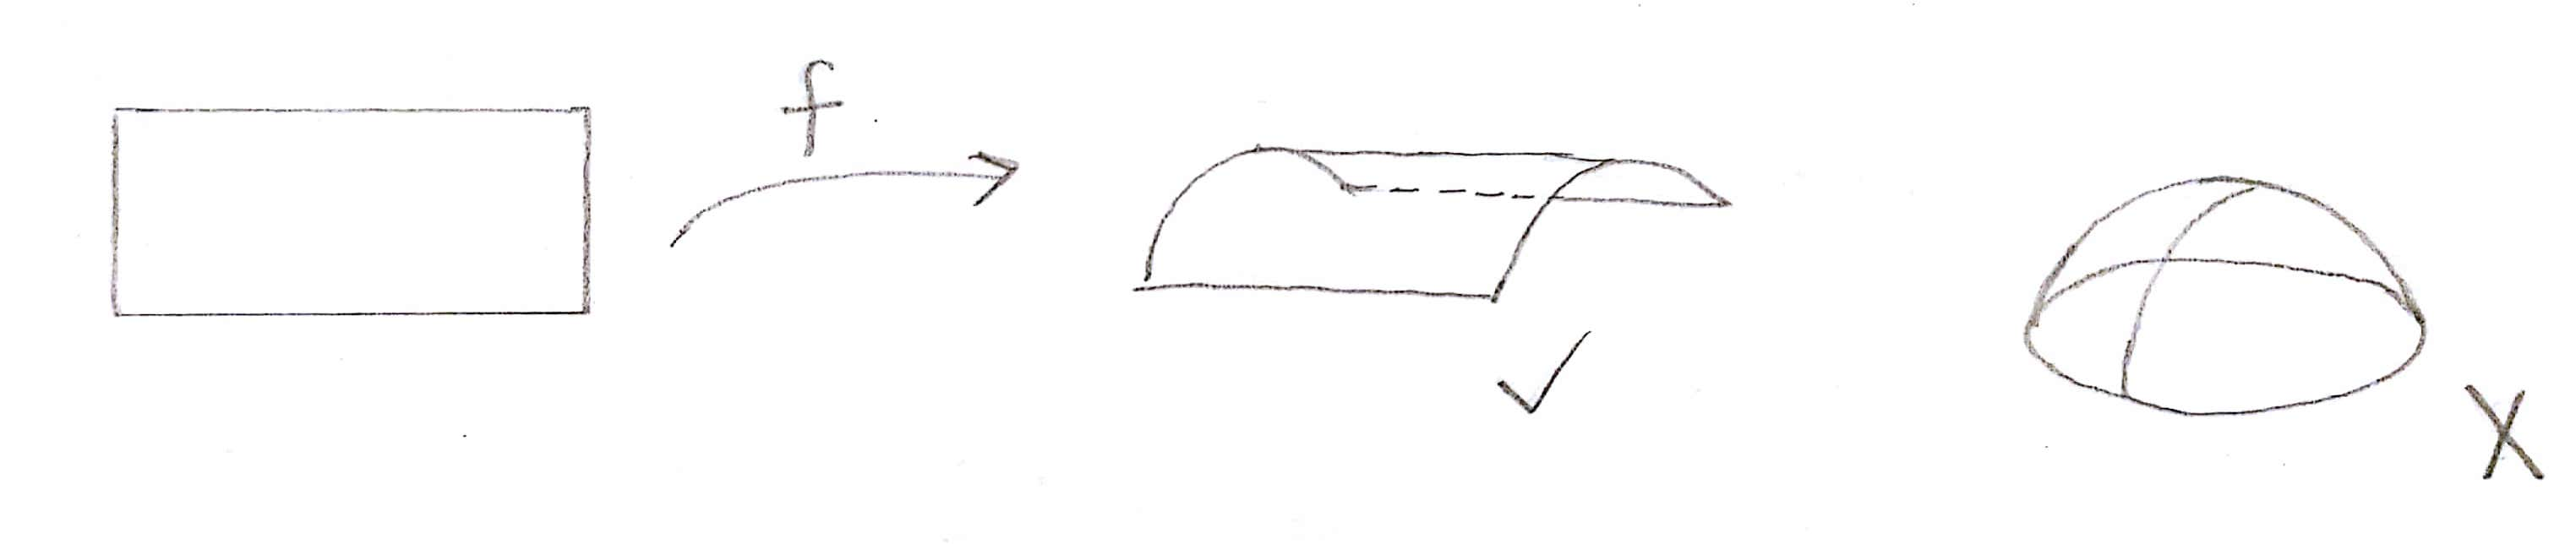
\includegraphics[width=1.0\textwidth]{chapter_7/files/isometric.jpeg}
\caption{The middle transformation has no stretch/shrink, but the rightmost transformation (a spherical cap) has stretch/shrink. }
\end{figure}
    
  \item Parametrization space should be convex. For example, if there
    is a missing/hole at the center of a manifold, an embedding will
    `fill in' the space and shorten the distance between two points
    that were originally across each other in the original manifold. 
  \end{itemize}

\end{itemize}

\subsection{LLE(Locally Linear Embedding)}
\subsubsection*{Goal}
Find a low-dimensional embedding that preserves ``local geometry". But
what is ``local geometry"? 

\textbf{Answer}: If a manifold is locally linear, one can define
``local geometry" as how a specific data point is linearly related to
its neighbors. Then we can find a low-dimensional embedding $Y$ of the
given data $X$ such that the locally linear relationships between
neighbors is approximately preserved. 

\subsection*{How?}
Input: Input data $X\in \mathbb{R}^{D\times n}$, number of neighbors
$k$, embedding dimension $d$. 
\begin{itemize}
\item Use the $k$-NN graph to find/determine the nearest neighbors for
  each data point $x_i$. 
\item 
\begin{align*}
&\min_{W} \Phi(W) = \sum_{i=1}^n \bigg|\bigg|x_i - \sum_{j\in N(i)}
  W_{ij} x_j\bigg|\bigg|^2\\ 
&\text{ s.t. } \forall i \ \sum_{j} W_{ij}=1.\\
&w_{ij}=0 \text{ where } j \not \in N(i)
\end{align*}
\item 
\begin{align*}
&\min_{Y} \Psi(Y) = \sum_{i=1}^{n} ||y_i - \sum_{j\in N(i)} W_{ij}
  y_i||^2\\ 
&\text{s.t. } Y Y^T = I 
\end{align*}
\end{itemize}


\subsection*{Details}
\subsubsection*{Step 2}
Consider the $i$-th data point. $\Phi (W_{i:})=||x_i-\sum_{j\in N(i)}
W_{ij} x_j||^2$.\\ 
We use the following notations:\\
$D\times k$ matrix:
\[N_i=
\begin{bmatrix}
    x_{j_1} & x_{j_2} & \dots & x_{j_k} \\
\end{bmatrix}
\]
$k\times 1$ vector:
\[W_i=
\begin{bmatrix}
    W_{ij_1} \\
    W_{ij_2} \\
    \vdots \\
    W_{ij_k} \\
\end{bmatrix}
\]
$k\times 1$ vector:
\[e=
\begin{bmatrix}
    1 \\
    1 \\
    \vdots \\
    1 \\
\end{bmatrix}
\]
So we can write the two parts as the following forms:
\[
\begin{bmatrix}
    x_i & x_i & \dots & x_i \\
\end{bmatrix} = x_i e^T
\]
\[
\Rightarrow x_i = x_i e^T w_i \text{ where } \sum_j w_{ij} = 1
\]
and
\[
\sum_{j\in N(i)} W_{ij} x_j=N_i W_i
\]
It follows that:
\begin{align*}
\min_{W_i} \Phi (W_{i:})
&= \min_{W_i} ||X_i e^T W_i - N_i W_i||^2\\
&= \min_{W_i} ||(X_i e^T-N_i)W_i||^2\\
&= \min_{W_i} W_i^T (X_i e^T-N_i)^T (X_i e^T - N_i)W_i
\end{align*}
The optimization now becomes:
\begin{align*}
&\min_{W_i} W_i^T G W_i \text{ where }G = (X_i e^T-N_i)^T (X_i e^T - N_i)\\
&\text{s.t. } e^T W_i = 1
\end{align*}
We relax the constraint using Lagrange and take the derivative of the
cost function as the following: 
\begin{align*}
L(W_i,\lambda) &= W_i^T G W_i - \lambda (e^T W_i - 1)\\
\frac{dL}{dW_i} &= 2GW_i - \lambda e = 0\\
2Gw_i &= \lambda e
\end{align*}
If $\lambda$ is known, $W_i=G^{-1} \frac{\lambda}{2} e$.\\
We can pick any $\lambda \neq 0$ and solve for $W_i$. $W_i^* =
\frac{W_i}{\sum_j W_{ij}}$. 

\subsubsection*{Step 3}
We use the following notations:\\
$d\times n$ matrix
\[
Y=
\begin{bmatrix}
    y_1 & y_2 & \dots & y_n \\
\end{bmatrix}
\]
\[
W=
\begin{bmatrix}
    \dots & \dots & \dots\\
    \dots & W_{ij} & \dots\\
    \dots & \dots & \dots\\
\end{bmatrix}
\]
\[
W_{:i}=
\begin{bmatrix}
    0 \\
    \vdots\\
    0\\
    W_{j_1}\\
    0\\
    \vdots\\
    0\\
    W_{j_2}\\
    0\\
    \vdots
\end{bmatrix}
\]
\[
I_{:i}=
\begin{bmatrix}
    0 \\
    \vdots\\
    0\\
    1 \text{ the }i\text{-th entry}
    0\\
    \vdots
\end{bmatrix}
\]
So we have
\[
y_i = y I_{:i}
\]
\[
\sum_{j\in N(i)} W_{:j} y_i = Y W_{:i}
\]
The optimization problem becomes:
\begin{align*}
&\min_{Y} \sum_{i=1}^n ||Y I_{:i} - Y W_{:i}||^2\\
&\min_{Y} ||Y I - Y W||_F^2\\
&\min_{Y} ||Y(I-W)||_F^2\\
&\min_Y tr((I-W)^T Y^T Y (I-W))\\
&\min_Y tr(Y(I-w)(I-W)^TY^T)\\
\end{align*}
It follows that:
\begin{align*}
&\min_Y \text{tr}(YMY^T)\\
&\text{s.t. } Y^TY=I
\end{align*}
where $M = (I-w)(I-W)^T$.\\
We can solve it by taking the eigenvalue decomposition takes
$2,3,...,d+1$ eigenvectors of $M$.\\ 
\subsubsection*{Observations}
\begin{itemize}
\item does not preserve the scale in the low-dimensional parametrization.
\item works quite poorly in practice.
\item $(I-W)(I-W)^T$ is kind of like a Laplacian of the underlying graph.
\end{itemize}

\subsection*{LE(Laplacian Eigenmaps)}
\subsubsection*{Goal}
Find a Low-Dimensional embedding of the original input data that
preserves "local geometry" in terms of maximally preserving similarity
between points. 
\textbf{Question}: How do we measure similarity?\\
\textbf{Answer}: Can estimate local distances define similarity
proportional to the distance. 
\subsubsection*{How?}
\begin{itemize}
\item Define $W_{ij}=e^{-||x_i-x_j||^2}{2\sigma^2}$.
\item 
\begin{align*}
&\min_{Y} \sum_{i,j} W_{ij} ||y_i-y_j||^2\\
&\text{s.t. } Y^T Y=I
\end{align*}
$\Rightarrow$
\begin{align*}
&\min_{Y} \text{tr} (Y^T LY)\\
&\text{s.t. } Y^T Y=I
\end{align*}
\end{itemize}
\subsubsection*{Observations}
If points $x_i$ and $x_j$ are far apart, $W_{ij}$ is close to 0 so
$y_i$ and $y_j$ can be mapped anywhere. If $x_i$ and $x_j$ are close,
then $w_{ij}$ is large so it encourages $y_i$ and $y_j$ to be mapped
close. In this sense, it is local neighborhood preserved. 

\subsection*{Discussion}
We can put most linear dimensionality reduction algorithms in a
unified framework. Essentially, they are all special cases of
Kernel-PCA. 
\begin{itemize}
\item PCA: $K=X^T X$(Linear Kernel).
\item Classical-MDS: $K=\frac{-1}{2} HD^{Euclidean}H$ where $H$ is the
  centering matrix. 
\item Isomap: $K=\frac{-1}{2} HD^{Geodesic}H$.
\item LLE: once $W$ is learned, $K=M^{-1}$ or $K=(\lambda_{max} I -
  M)$, where $M=(I-W)(I-W)^T$. (Difference is in the scale of
  coordinate of the embedding. $K=\wedge^{1/2} V$). 
\item LE: $K=L^{-1}$ or $K=(\lambda_{max} I - L)$ and the result is
  also off in the scale of coordinate of the embedding as LLE. 
\end{itemize}

\subsection*{MVU(Maximum Variance Unfolding) (aka. Semi-Definite Embedding(SDE))}
\subsubsection*{Goal} Find a low-dimensional embedding of the given
data which preserves "local geometry" in terms of finding the best
kernel.\\
Define Local Geometry in terms of distance between data points in a
local neighborhood. Denote $D\times n$ matrix
\[
X=
\begin{bmatrix}
    x_1 & x_2 & \dots & x_n \\
\end{bmatrix}
\]
and denote $d\times n$ matrix
\[
Y=
\begin{bmatrix}
    y_1 & y_2 & \dots & y_n \\
\end{bmatrix}.
\]
Want: If $j$ is a neighbor of $i$,
\begin{itemize}
\item \begin{align*}
||x_i - x_j||^2
&=||\phi (x_i)-\phi (x_j)||^2\\
&=K_{ii}+K_{jj}-2K_{ij}
\end{align*}.
\item $K$ is positive semi-definite.
\item $\sum_{ij} K_{ij}=0$.
\end{itemize}

The optimization problem can be formulated as the following:
\begin{align*}
&\max_{K} \text{tr}(K)\\
&\text{s.t. } K_{ii}+K_{jj}-2K_{ij}-||x_i-x_j||^2 \text{ if }i \text{
    and } j \text{ are neighbors}.\\ 
&\text{s.t. } \sum_{ij}K_{ij}=0\\
&\text{s.t. } K \succeq 0
\end{align*}
This is a convex optimization and can find a globally optimal solution.

\subsection*{More discussions}
Suppose we want to preserve geodesic distance approximately.
\begin{theorem}[JL-manifold]
Say n-dimensional manifold $M$ in $\mathbb{R}^D$. We know that the
volume of the manifold, Vol$(M)=V$ and global bound on curvature
$K(M)=k$. $\exists f: \mathbb{R}^D \rightarrow \mathbb{R}^d$ where
$d=O(\frac{n}{\epsilon^2}\log (Vk) )$. $\forall p,q \in M$ and
$G(p,q)$ is the geodesic path between $p,q$. Let $L(\cdot)$ be the
"length" function. $\forall p,q,n$, 
\[
1-\epsilon \leq \frac{L(G(f(p),f(q)))}{L(G(p,q))} \leq 1+\epsilon
\]
$f$ is linear (can use random projection matrix).
\end{theorem}
